\section{Konzept}

\subsection{UseCase}
\begin{figure}[H]
  \begin{center}
    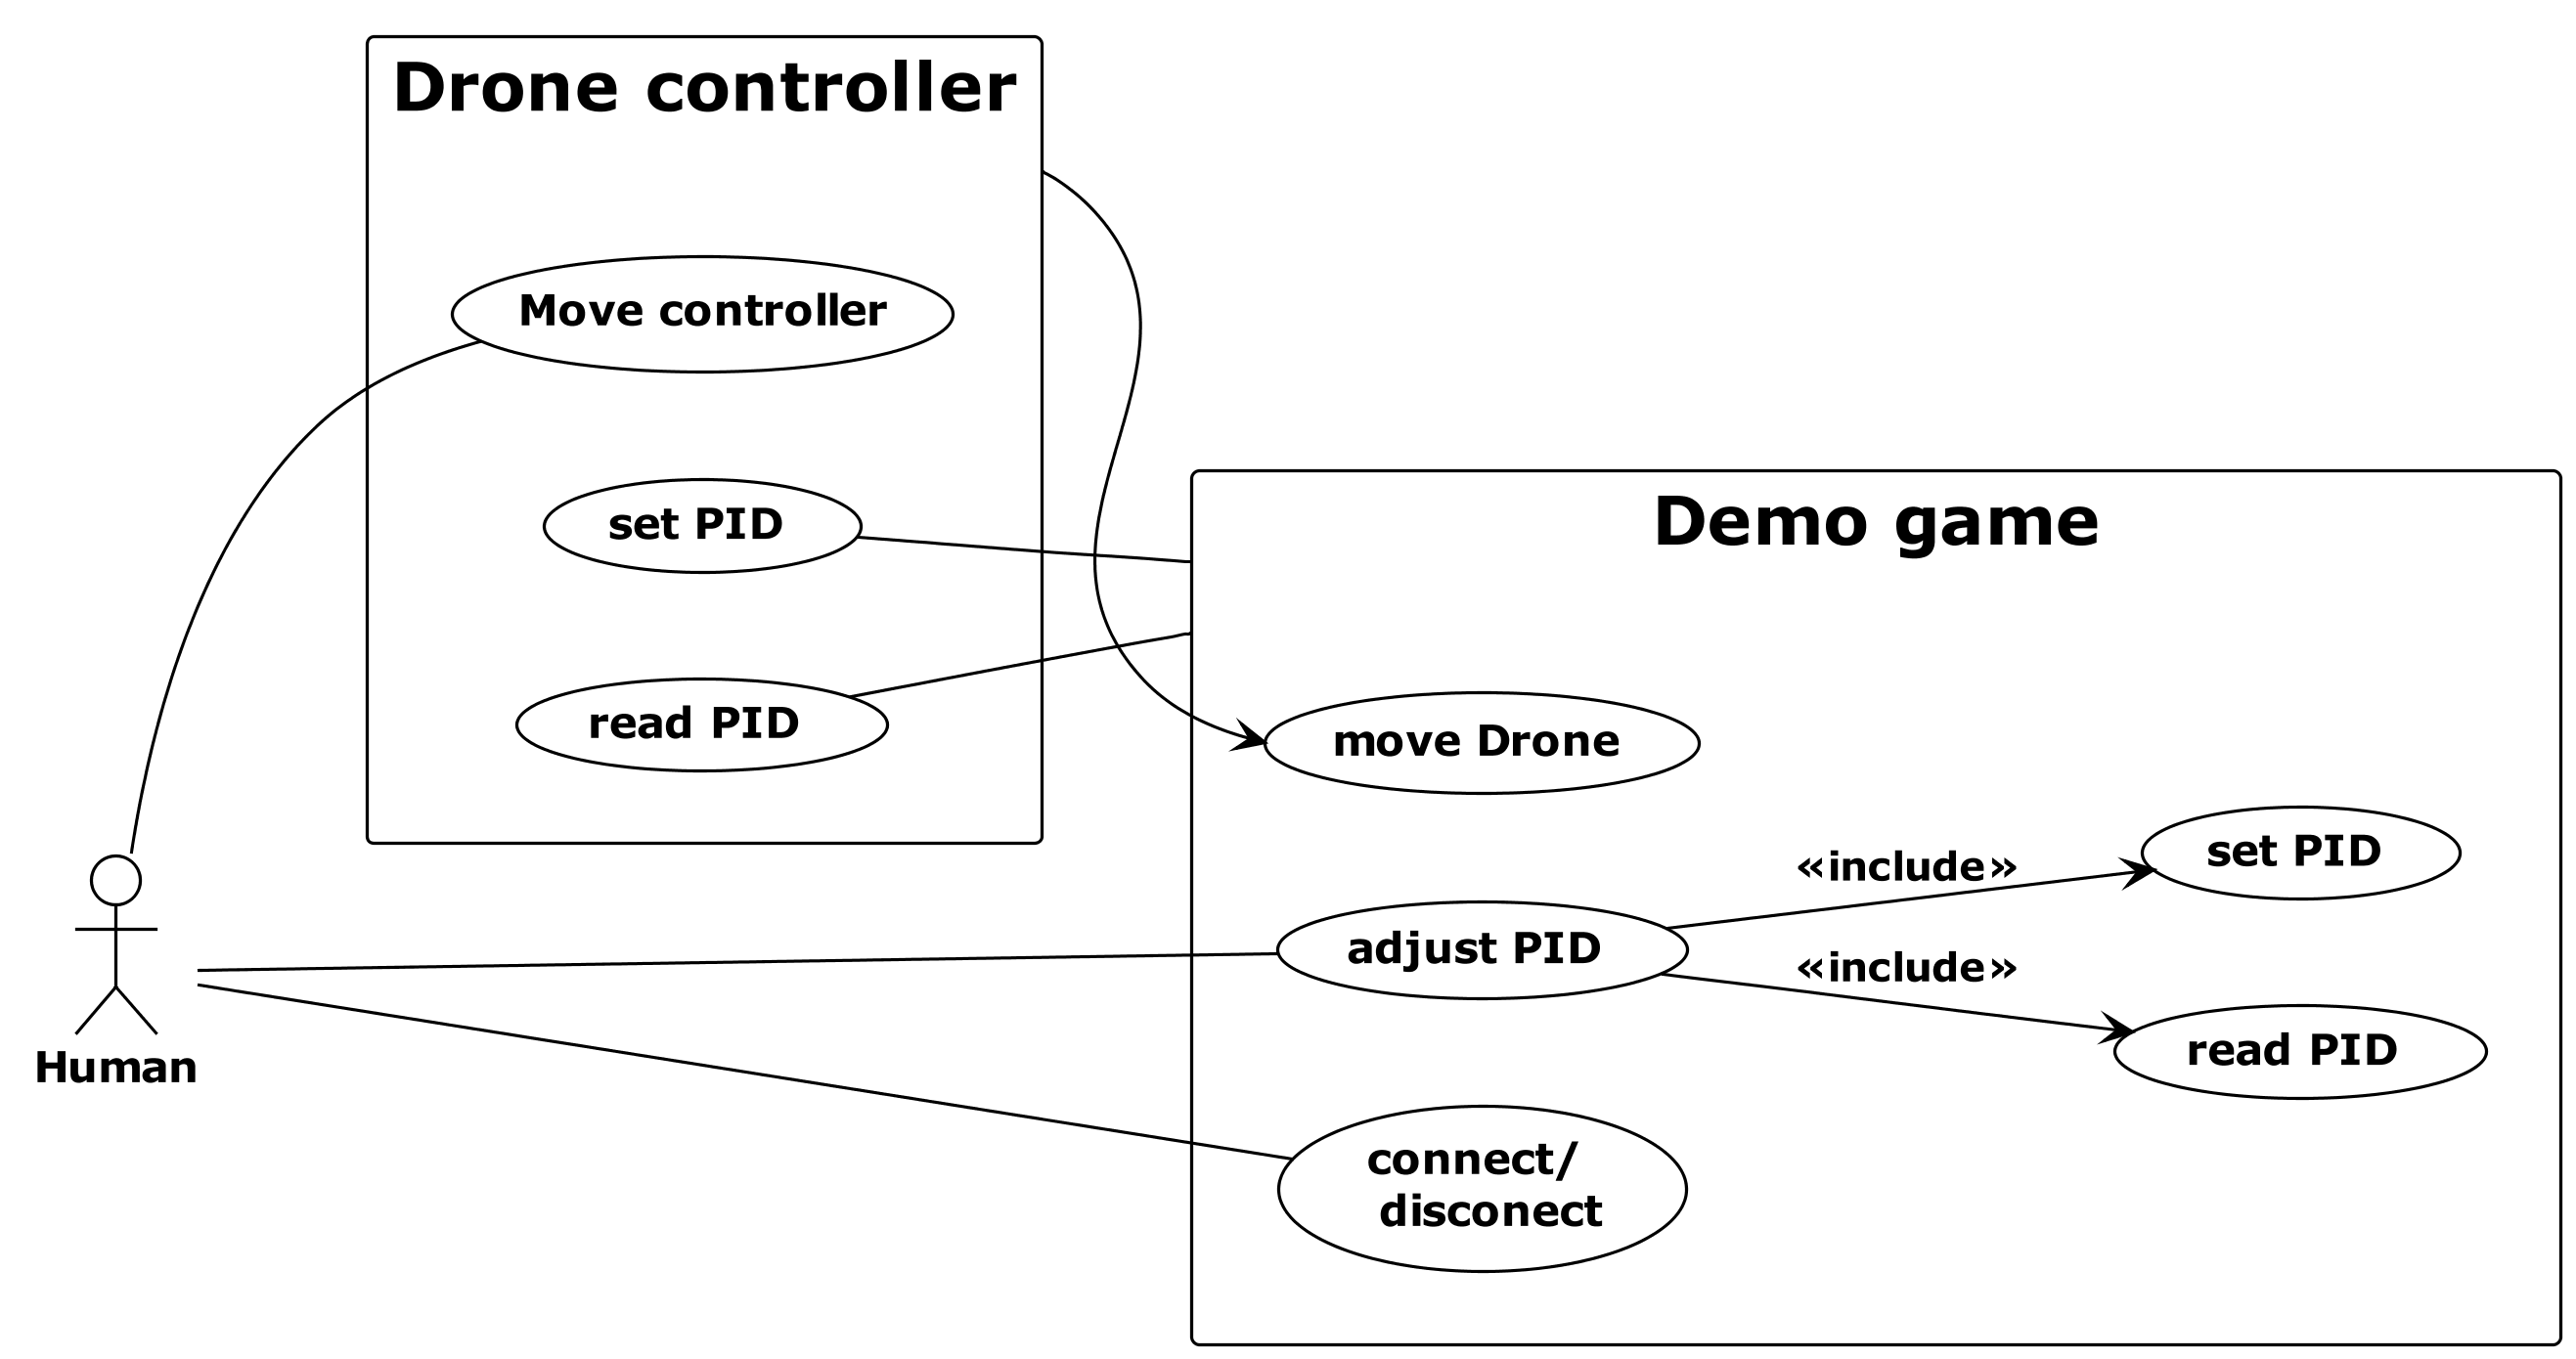
\includegraphics[width=0.9\linewidth]{content/diagrams/out/usecase/usecaseControl.png}
    \caption{UseCase Drohnensteuerung}
  \end{center}
\end{figure}

\subsection{Sequenzdiagramme}
\begin{figure}[H]
  \begin{center}
    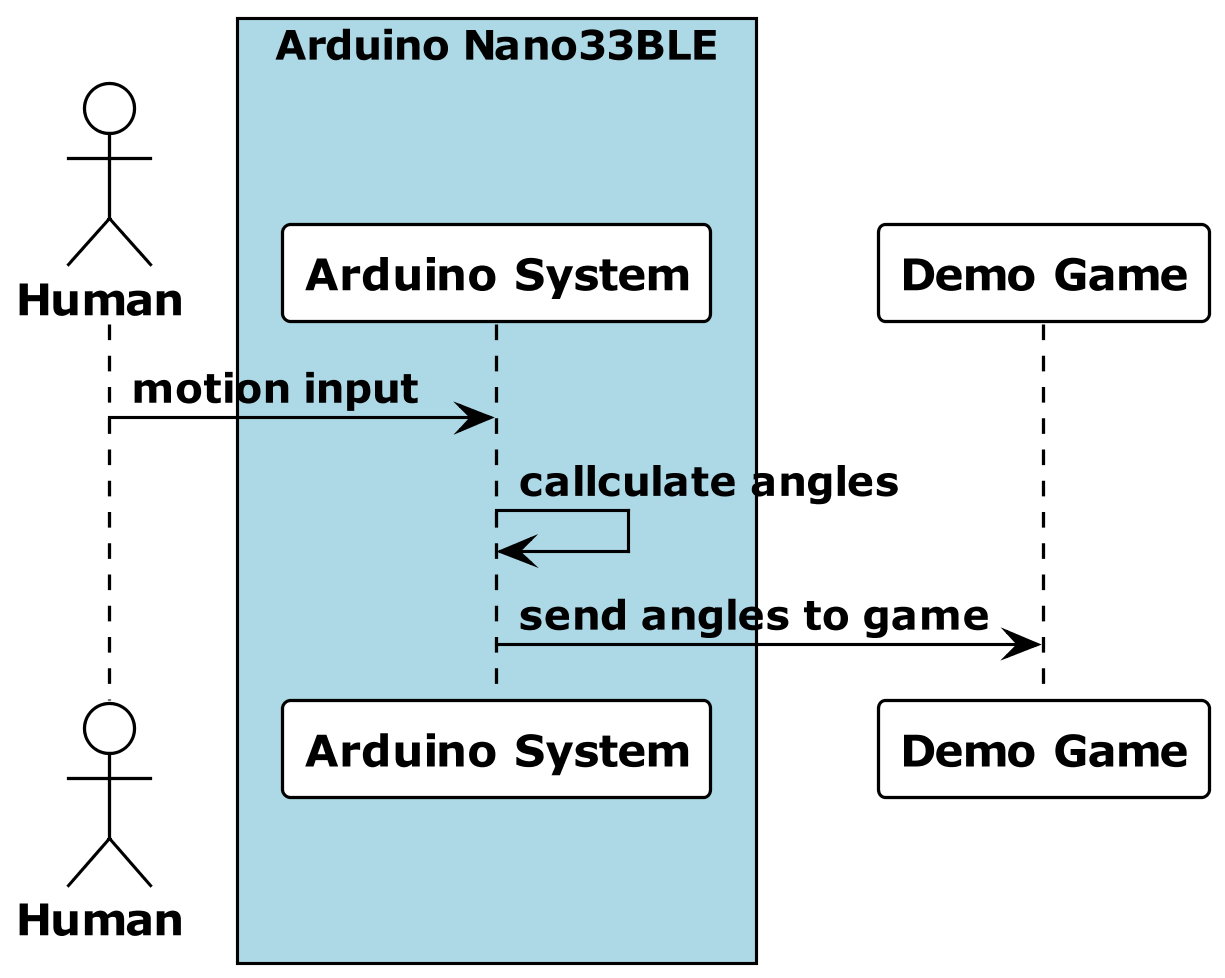
\includegraphics[width=0.5\linewidth]{content/diagrams/out/sequence/system.png}
    \caption{System}
  \end{center}
\end{figure}

\begin{figure}[H]
  \begin{center}
    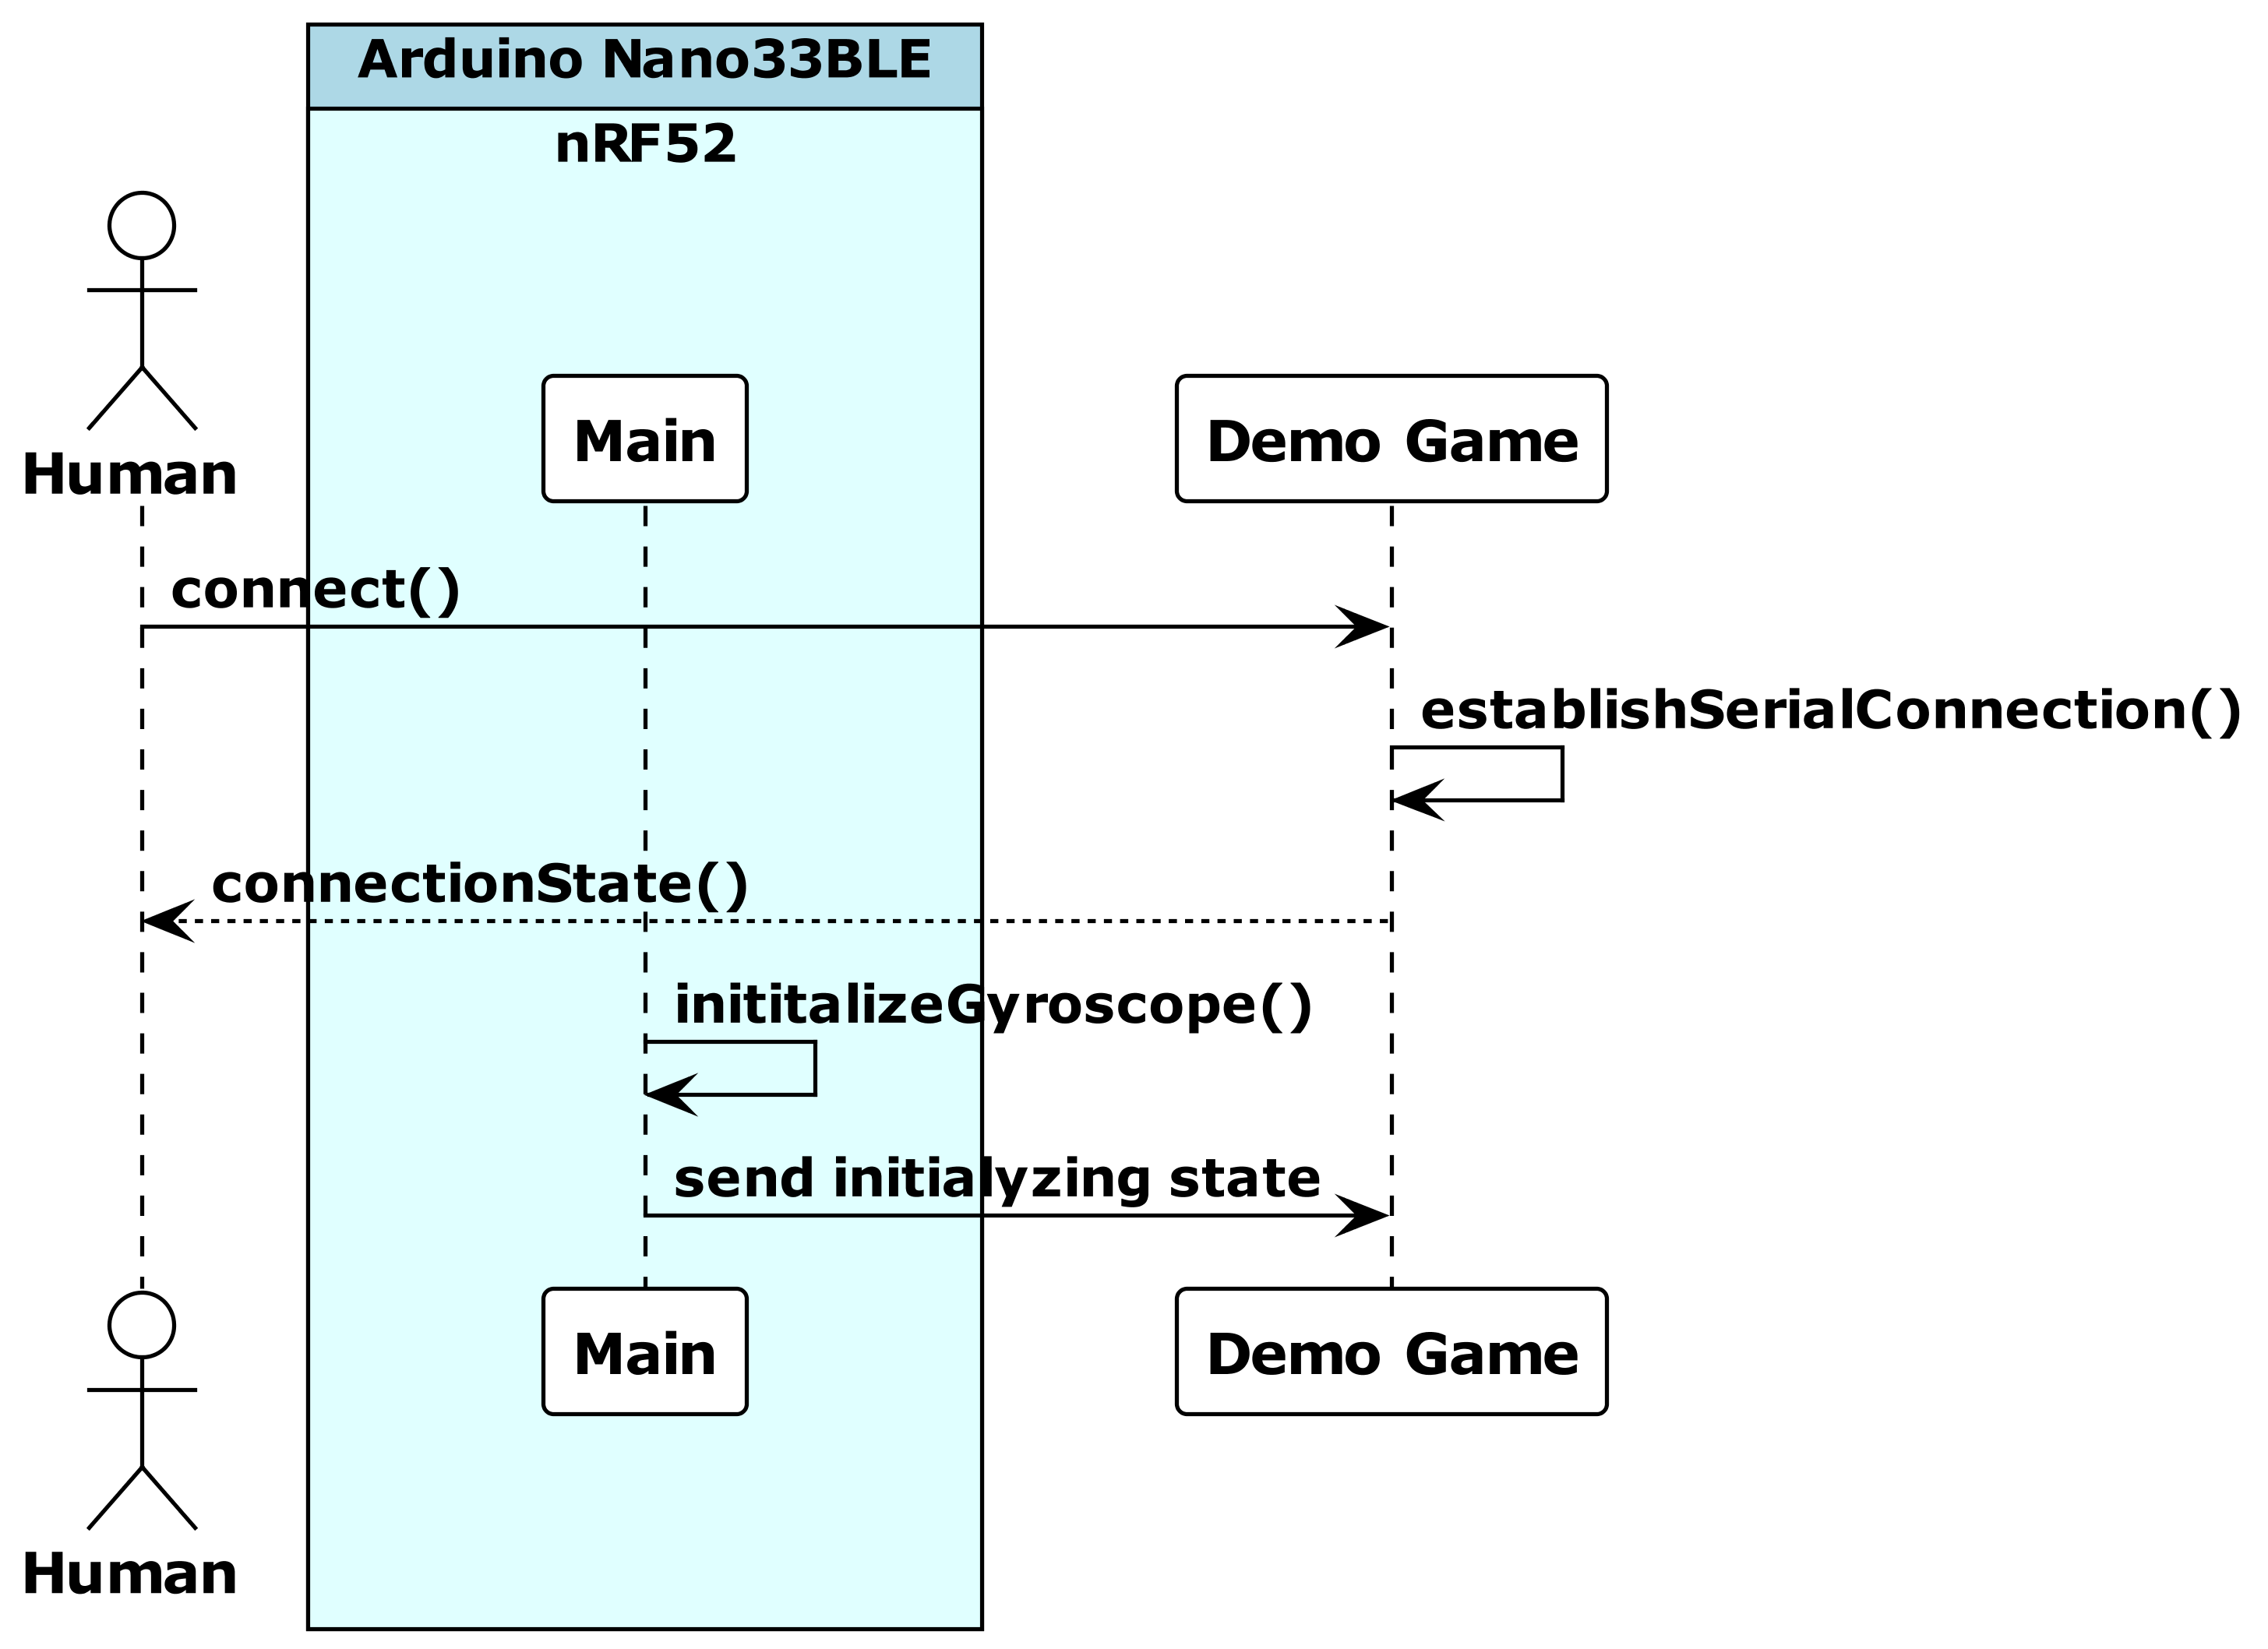
\includegraphics[width=0.7\linewidth]{content/diagrams/out/sequence/connect.png}
    \caption{Verbindung herstellen}
  \end{center}
\end{figure}

\begin{figure}[H]
  \begin{center}
    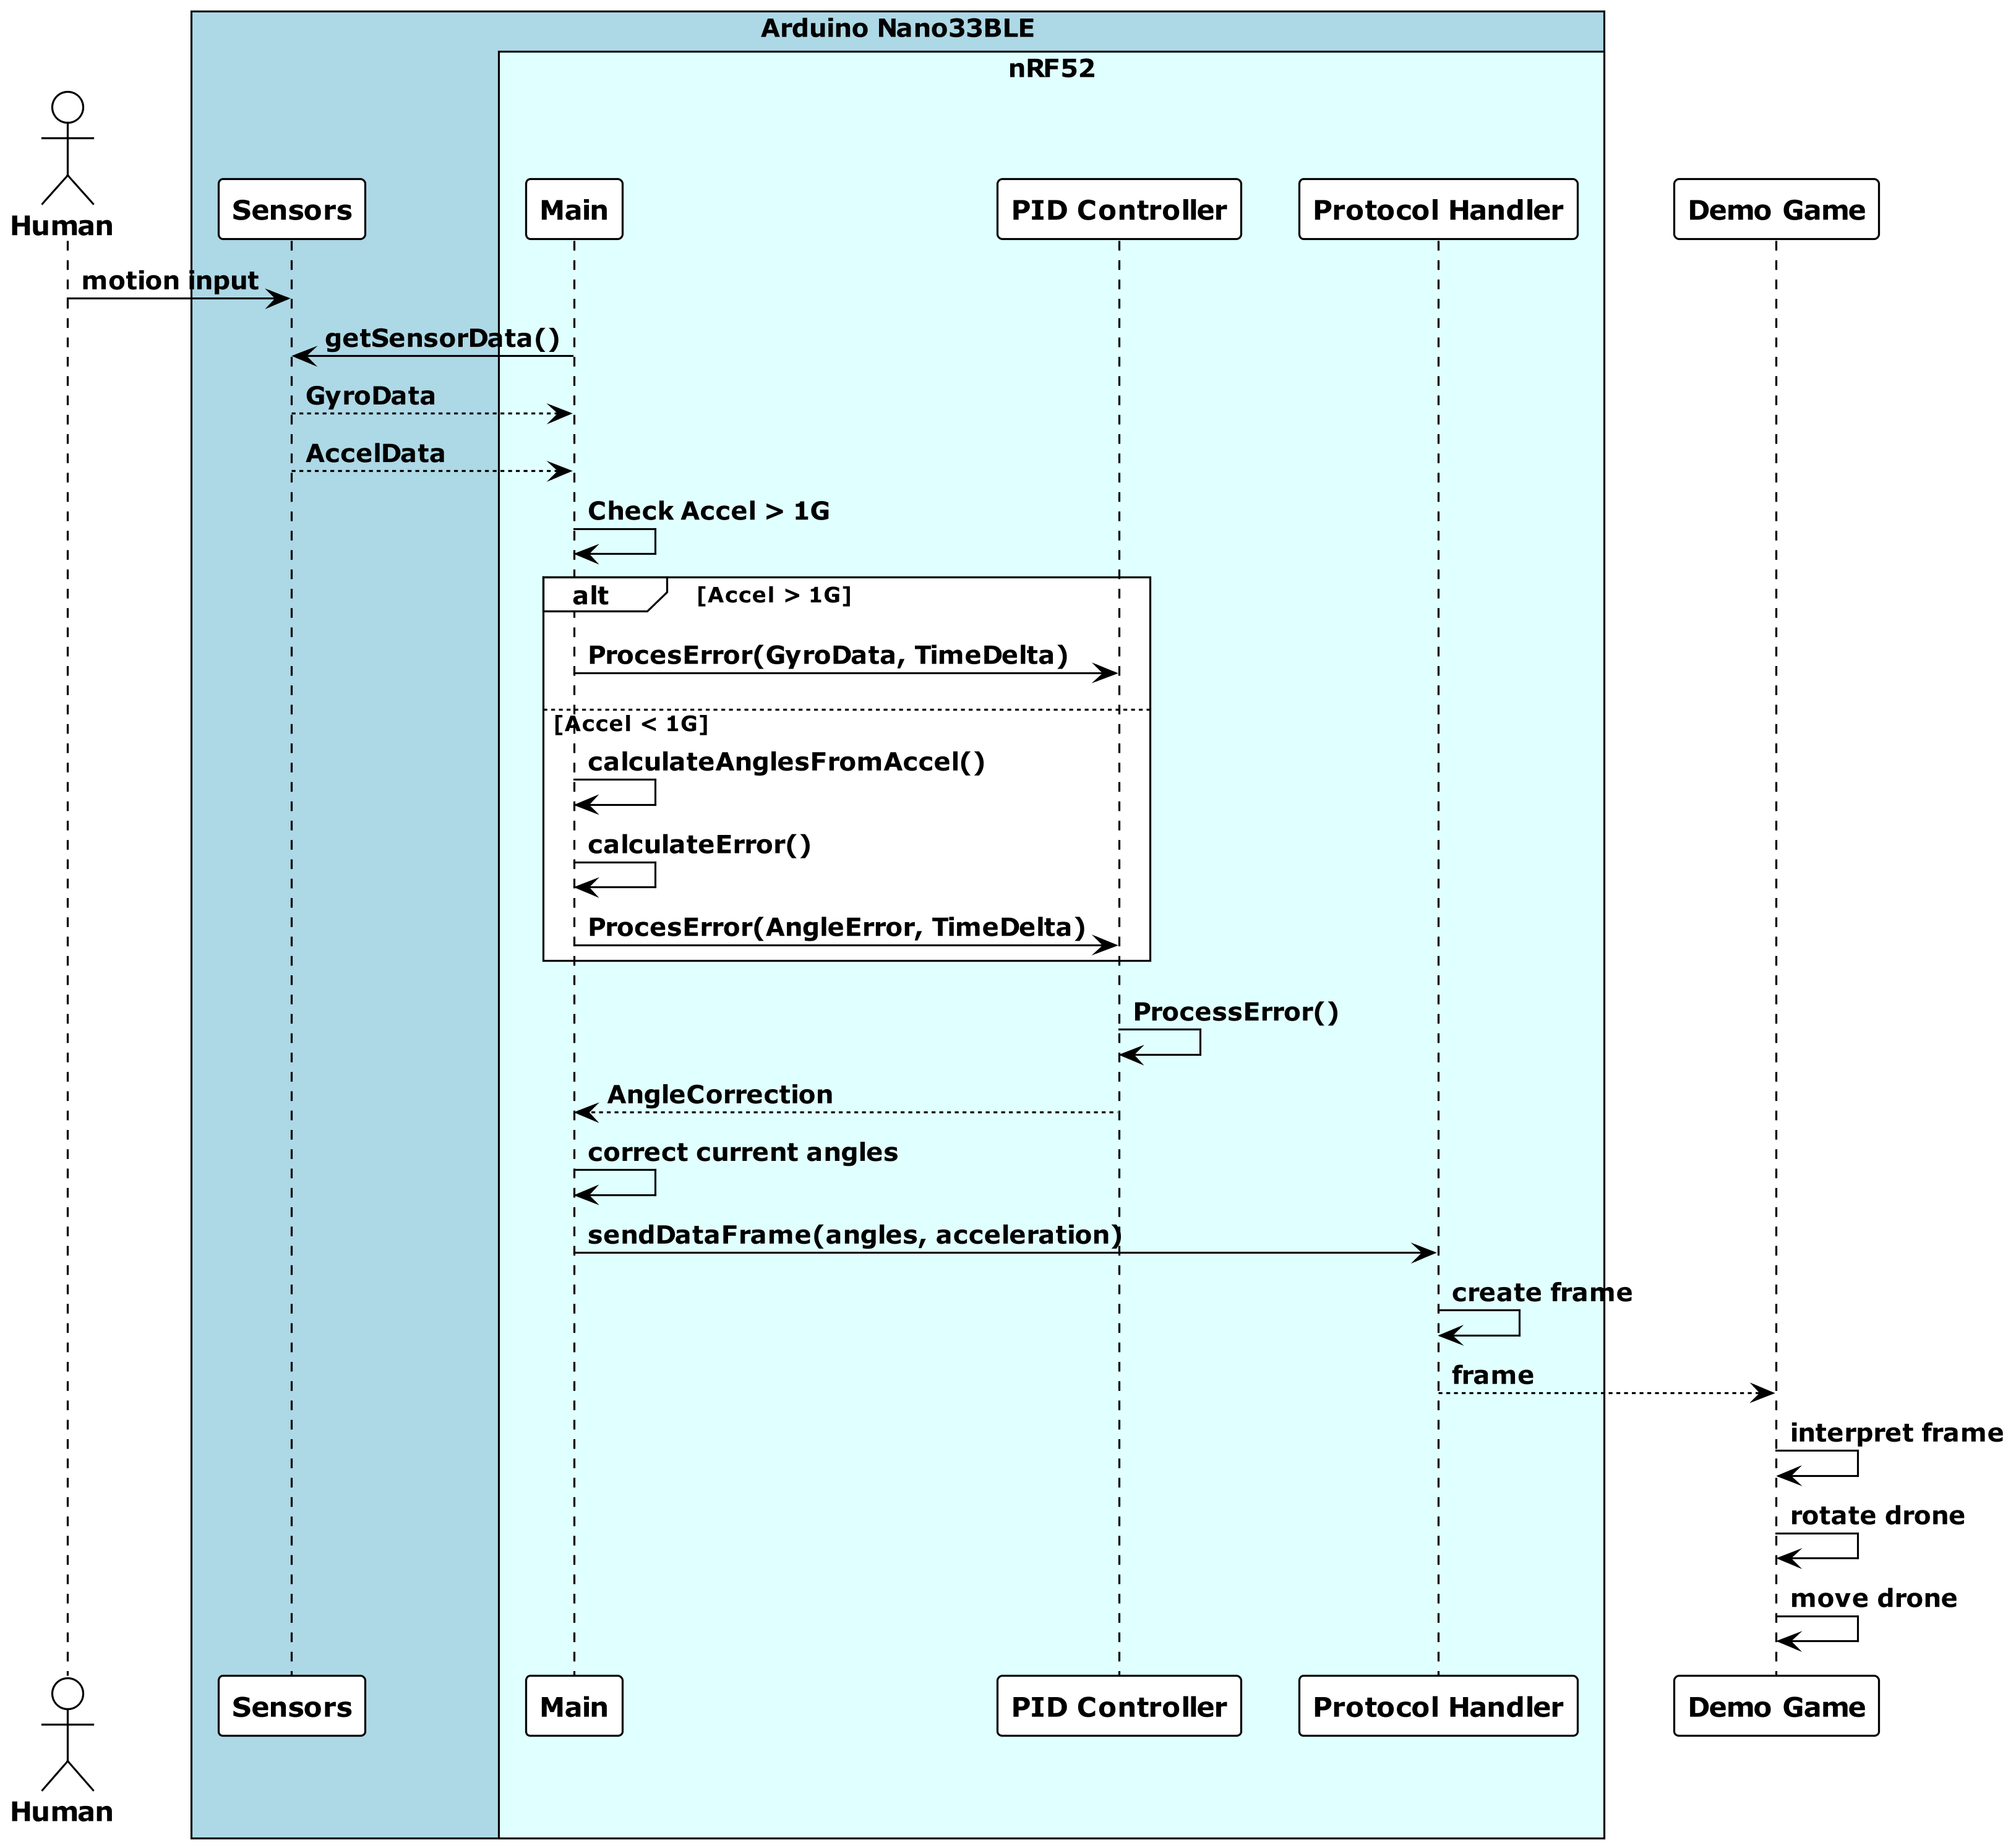
\includegraphics[width=1\linewidth]{content/diagrams/out/sequence/moveController.png}
    \caption{Move controller}
  \end{center}
\end{figure}

\begin{figure}[H]
  \begin{center}
    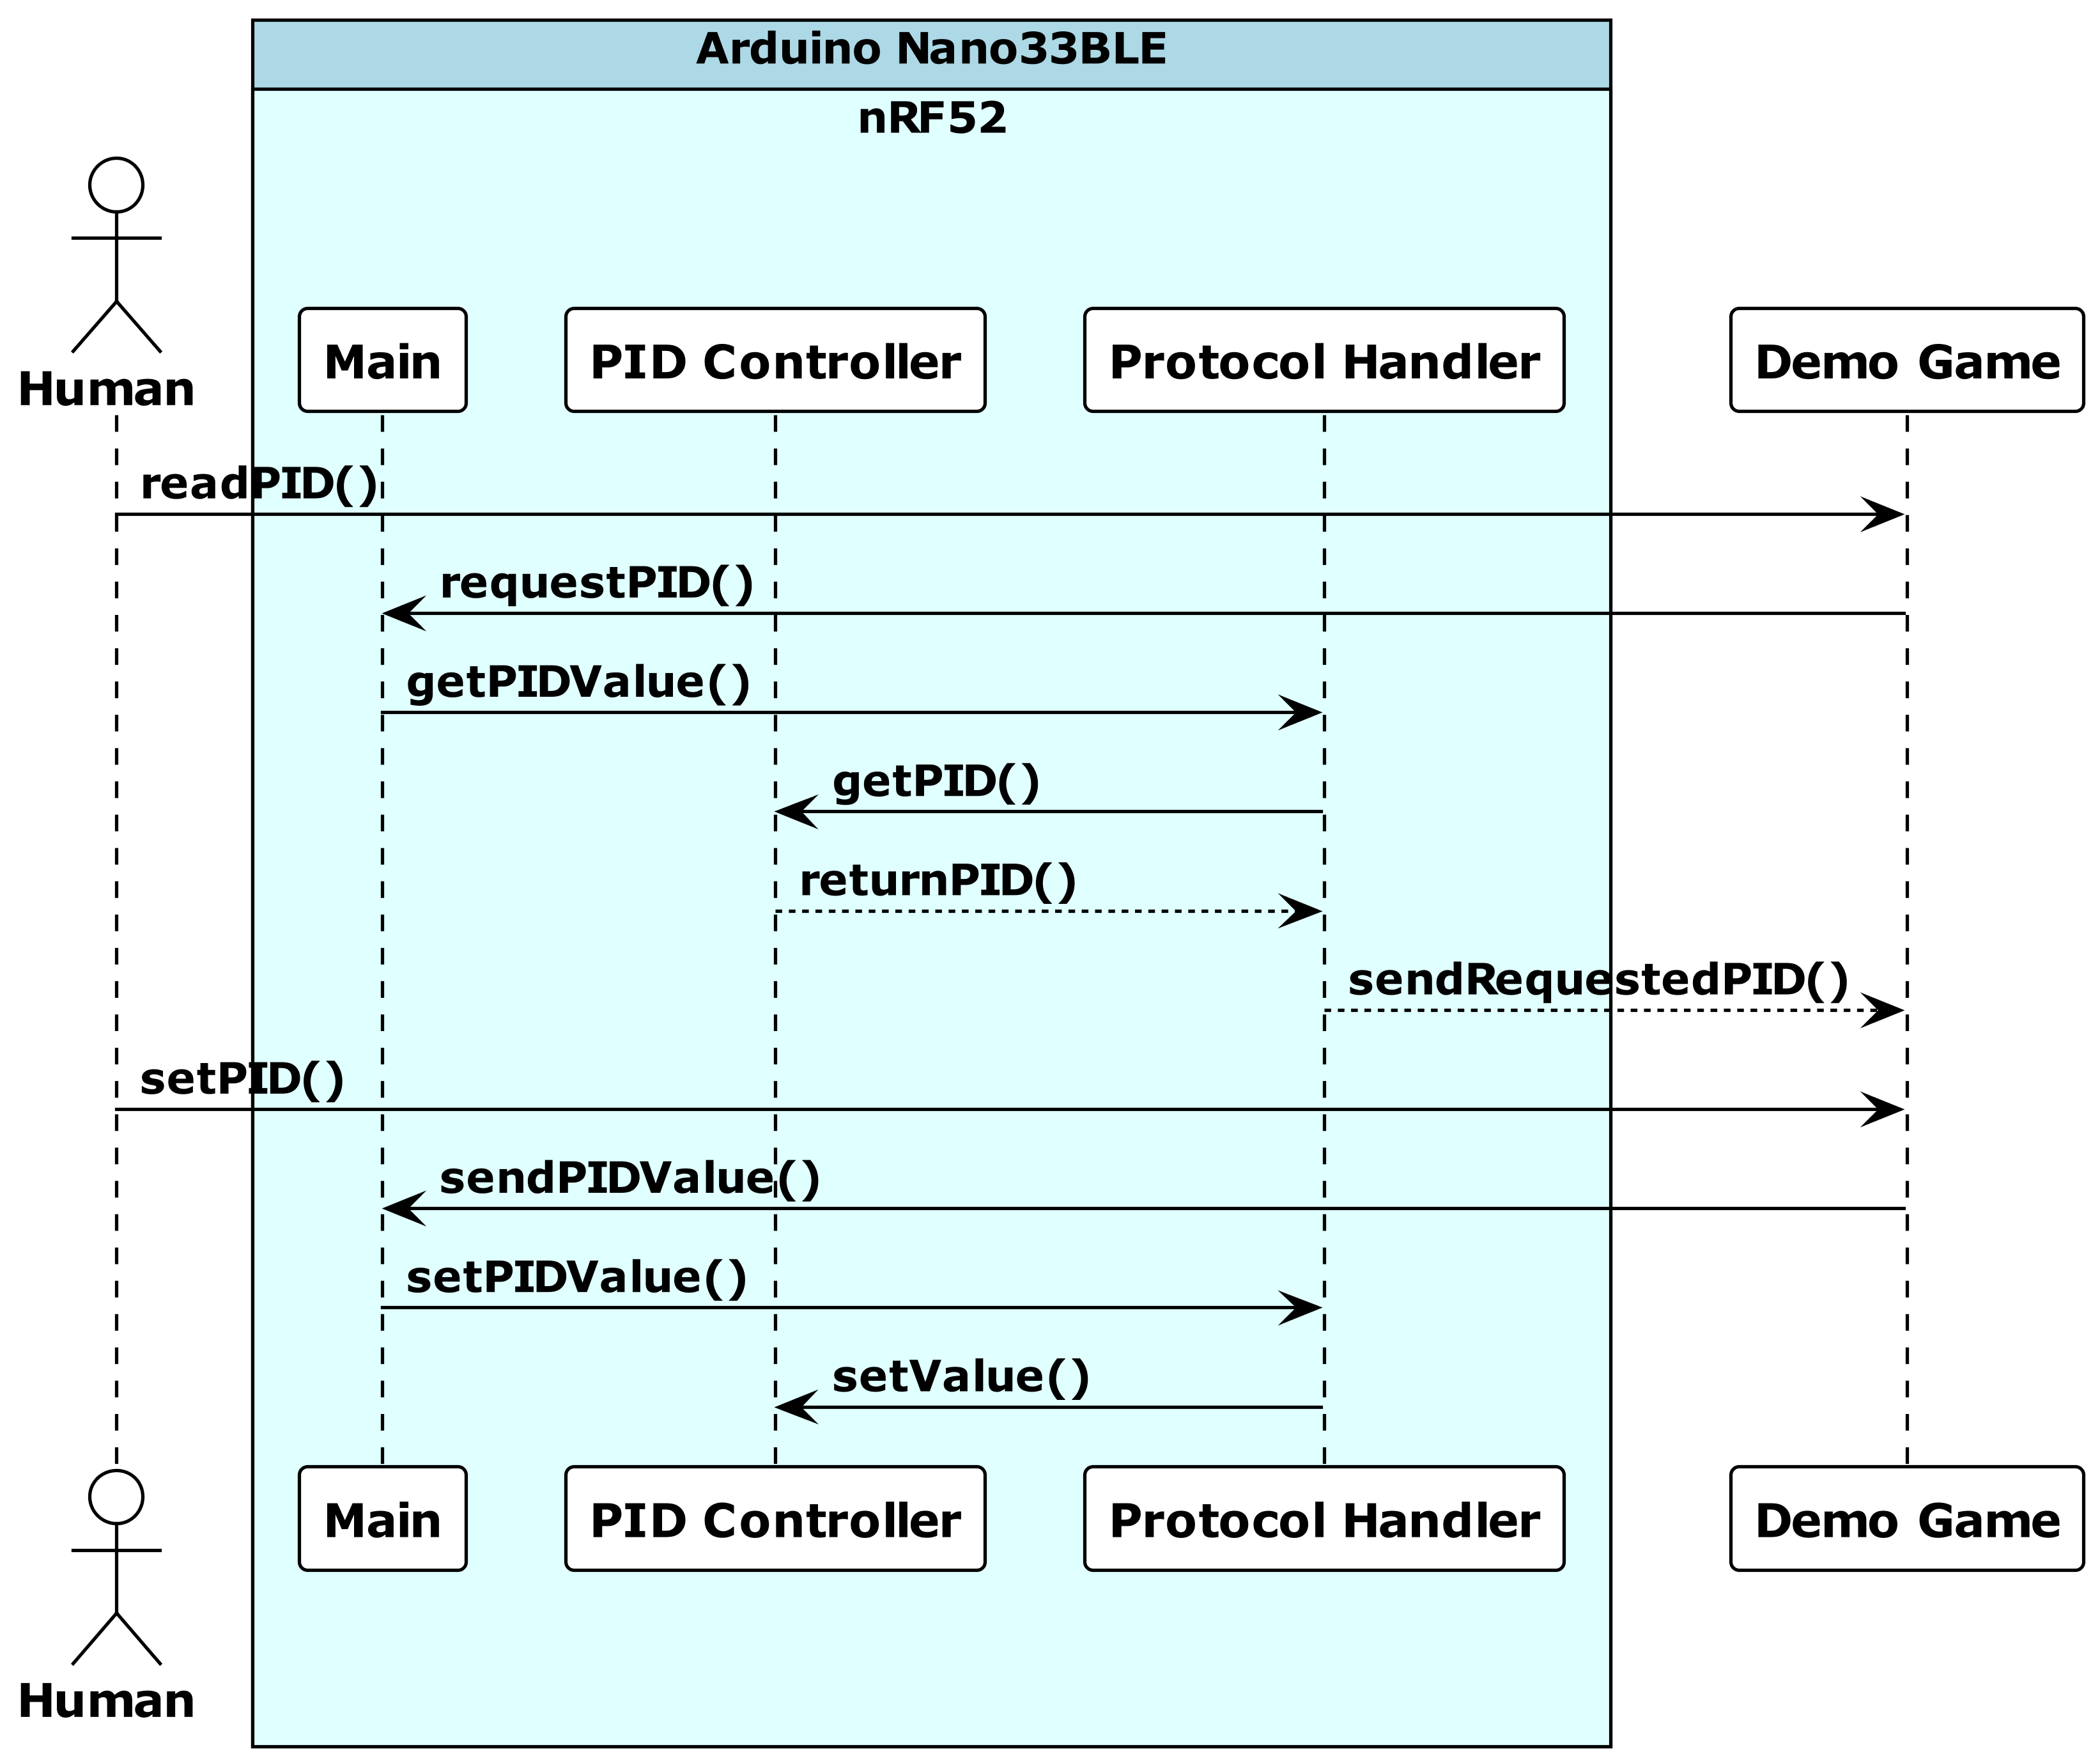
\includegraphics[width=0.7\linewidth]{content/diagrams/out/sequence/adjustPID.png}
    \caption{Adjust PID}
  \end{center}
\end{figure}

\subsection{Klassendiagramm}
\begin{figure}[H]
  \begin{center}
    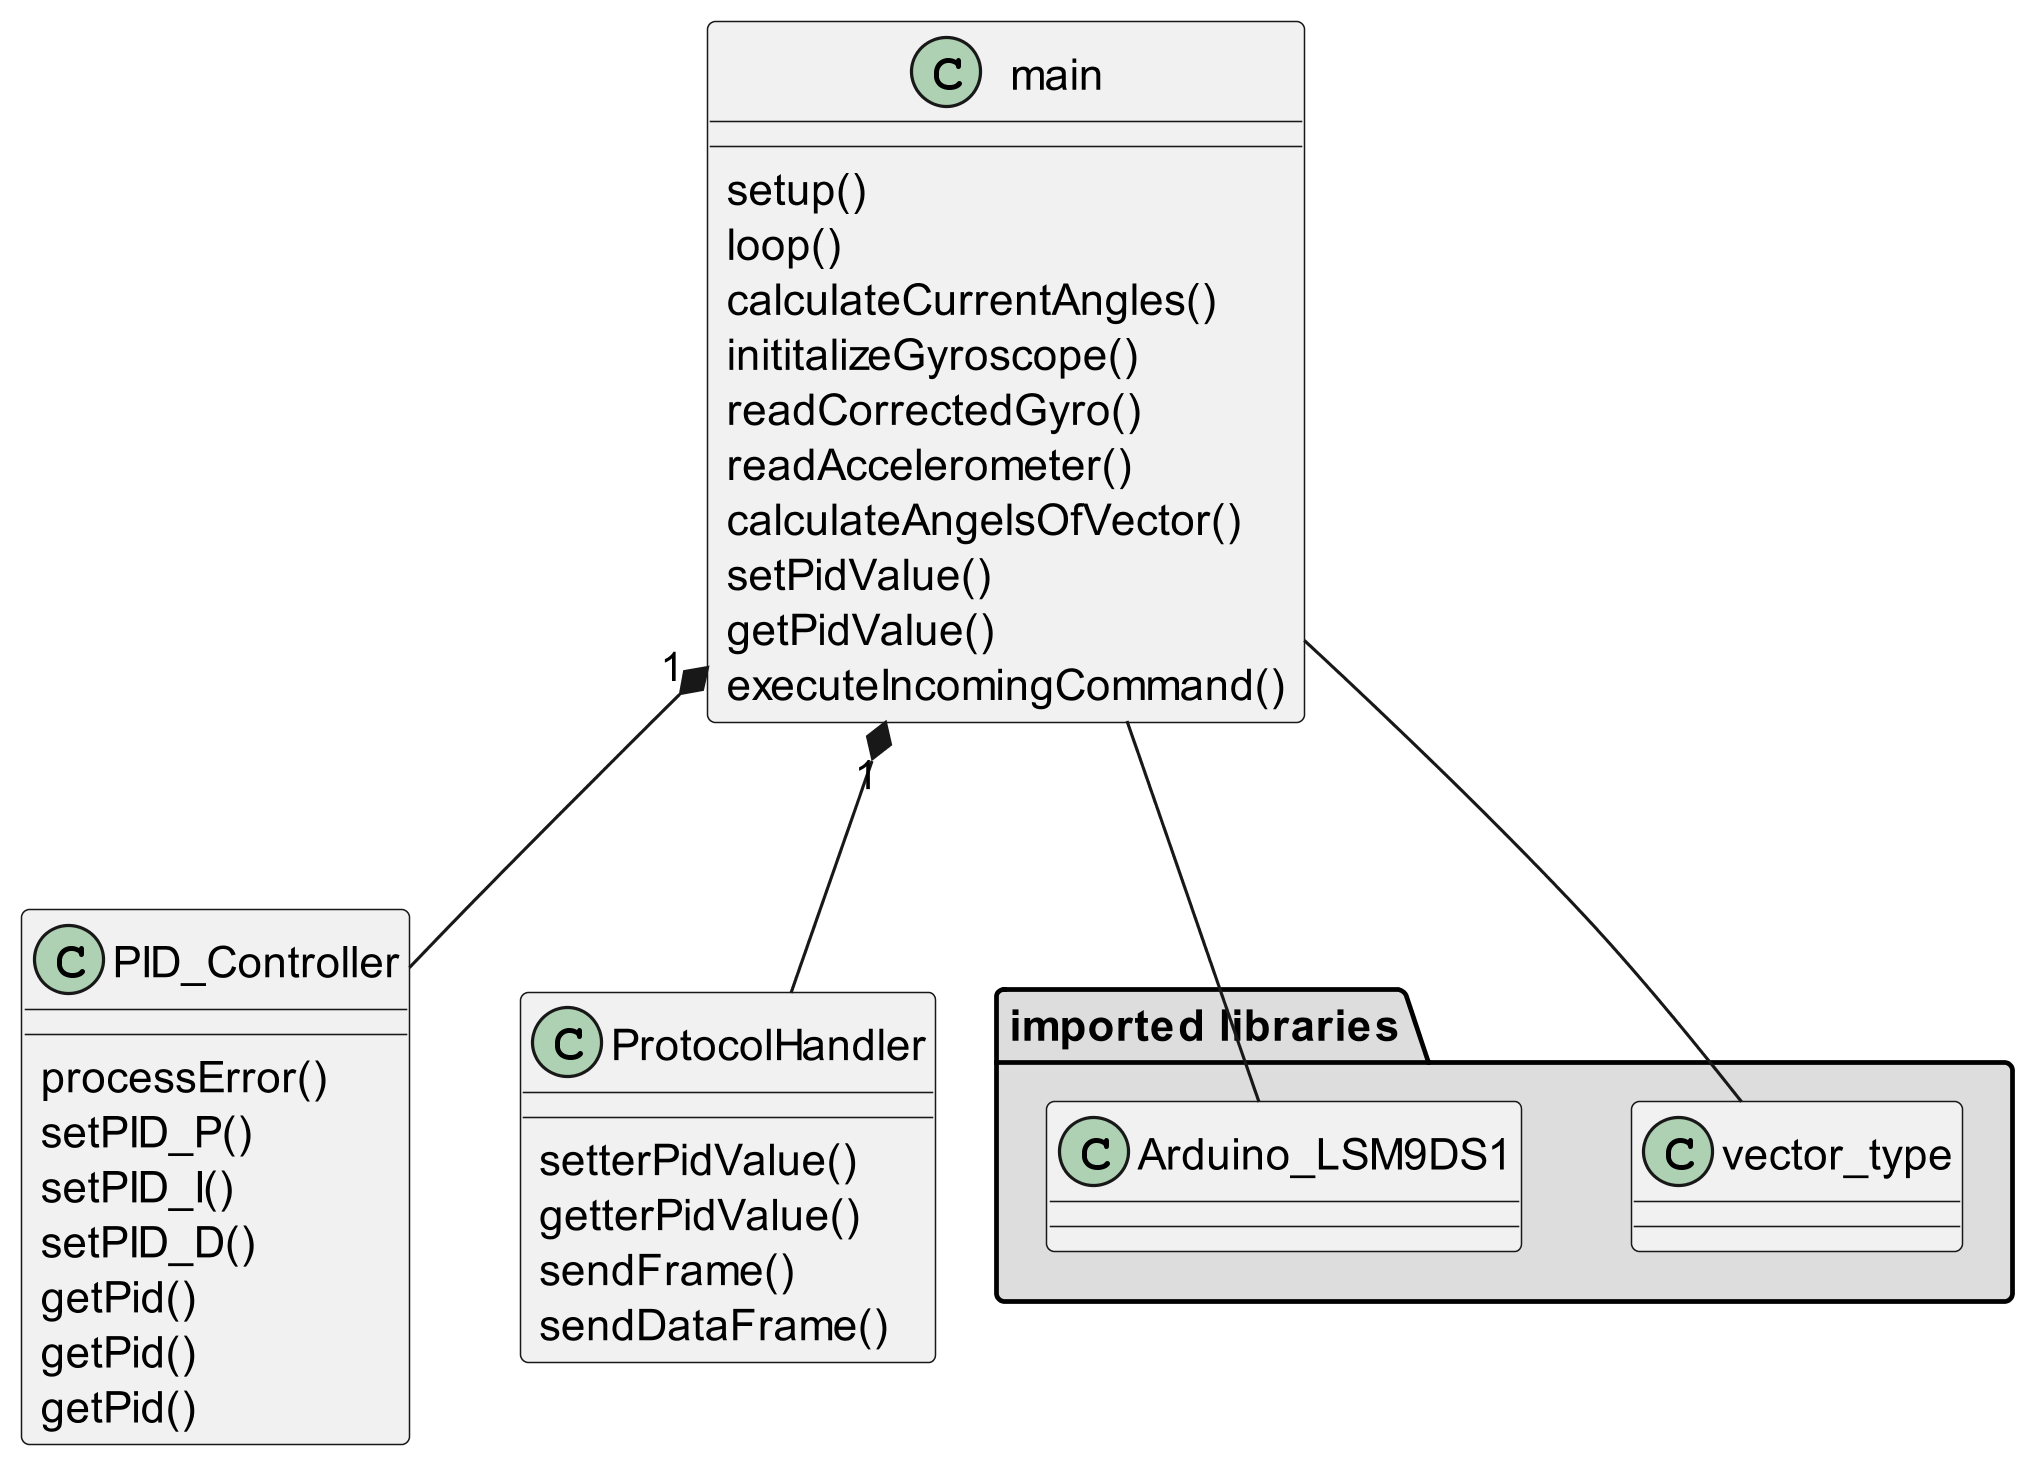
\includegraphics[width=0.8\linewidth]{content/diagrams/out/class/classdiagram.png}
    \caption{Klassendiagramm}
  \end{center}
\end{figure}

\subsection{Beschreibung der Klassen und Funktionen}
In diesem Kapitel werden die benutzten Klassen und deren Funktion kurz beschrieben.
\subsubsection{Vector\_type}
Bibliothek für 3D-Vektoren und Quaternionen. Einfache Bibliothek, die Strukturen für einen 3D-Vektor und eine 4D-Quaternion enthält. Alle grundlegenden Operationen sind zusammen mit Rotationen enthalten.

\subsubsection{Arduino\_LSM9DS1}
Bibliothek um die Accelerometer, Magnetometer und gyroscope Daten des LSM9DS1 IMU vom Arduino auszulesen. Die Magnetometer-Daten haben wir für dieses Projekt nicht verwendet.


\subsubsection{''main'' Klasse}
Die ''main'' Klasse ist die hauptklasse welche alle anderen Klassen Importiert. Hier befindet sich ebenfalls die setup() Funktion und die loop() Funktion welche im Arduino vorgeben sind.

\begin{table}[H]
  \centering
  \settowidth\tymin{executeIncomingCommand()}
  \setlength\extrarowheight{2pt}
  \begin{tabulary}{1.0\textwidth}{|L|L|}
    \hline
    \textbf{Funktion} &
    \textbf{Beschreibung}\\
    \hline
    setup() &
    Setupfunktion des Arduino. Wird ausgeführt wenn der Arduino gestartet wird.\\
    \hline
    loop() &
    Der Loop ist eine Endlosschleife, der nach jedem Durchlauf erneut aufgerufen wird.\\
    \hline
    initializeGyroscope() &
    Mit dieser Funktion wird das Gyroskop beim einschalten initialisiert und kalibriert.\\
    \hline
    readAccelerometer() &
    \\
    \hline
    readCorrectetGyro() &
    \\
    \hline
    calculateCurrentAngles() &
    \\
    \hline
    calculateAnglesOfVector() &
    \\
    \hline
    executeIncomingCommand() &
    Diese Funktion wertet den eingegangenen Befehl aus und führt anschliessend die entsprechende Funktion aus.\\
    \hline
    setPidValue() &
    Wird aus executeIncomingCommand() aufgerufen und setzt die eingegangenen PID-Werte über den PID Controller.\\
    \hline
    getPidValue() &
    Wird aus executeIncomingCommand() aufgerufen und sendet die angeforderten PID Werte zurück.\\
    \hline
  \end{tabulary}
  \caption{Beschreibung der ''main'' Klasse}
\end{table}

\subsubsection{PID Controller}
Die PID Controller werden zur glättung der Sensorsignale verwendet.\\
Je nach Situation, wird aus den Gyroskop oder Beschleunigungsdaten ein Fehler berechnet. 
Dieser Fehler beschreibt die Diskrepanz zwischen der theoretischen und der von den Sensoren ausgelesenen Orientation des Boards.
Mit Hilfe der PID Controller wird nun die theoretische Orientation entsprechend den Sensordaten angepasst.
Der PID-Algorythmus wird hier als eine Art Filter eingesetzt und glättet somit fehlerhafte Sensordaten etwas aus.\
\begin{table}[H]
  \centering
  \settowidth\tymin{processError()}
  \setlength\extrarowheight{2pt}
  \begin{tabulary}{1.0\textwidth}{|L|L|}
    \hline
    \textbf{Funktion} &
    \textbf{Beschreibung}\\
    \hline
    processError() & Ein Fehler wird als Input eingegeben und durchläuft den PID Algorythmus\\
    \hline
    setPID\_() & Setzt den eingehenden Wert einsprechend für P, I oder D. \\
    \hline
    getPID\_() & Sendet den aktuellen P,I oder D- Wert zurück.\\
    \hline
  \end{tabulary}
  \caption{Beschreibung PIDController}
\end{table}


\subsubsection{ProtocolHandler}
Mit dem ProtocolHandler wird das sende und empfangsprotokoll zum Steuern der Gamedemo kontrolliert.
\begin{table}[H]
  \centering
  \settowidth\tymin{sendPIDToSerial()}
  \setlength\extrarowheight{2pt}
  \begin{tabulary}{1.0\textwidth}{|L|L|}
    \hline
    \textbf{Funktion} &
    \textbf{Beschreibung}\\
    \hline
    setterPidValue() &
    Wertet den eingegangen Befehl zum setzen des PID-Werts aus und führt dann die entsprechende Funktion über den PIDController aus. \\
    \hline
    getterPidValue() &
    Wertet den eingegangen Befehl zum lesen des Aktuellen PID-Werts aus, holt sich den wert über den PIDController und sendet diesen über die Funktion sendPIDToSerial() zurück.\\
    \hline
    sendPIDToSerial() & 
    Wird durch getterPIDValue() aufgerufen und sendet PID-Wert über Serial.println() als string zurück.\\
    \hline
    sendDataFrame() &
    Wird durch den loop() aufgerufen und sendet die berechneten Gyro- und Beschleunigungsdaten Serial.println() als string an das Demo-Game.\\
    \hline
  \end{tabulary}
  \caption{Beschreibung ProtocolHandler}
\end{table}

\newpage